\documentclass[ngerman]{gdb-aufgabenblatt}

\usepackage{weiwBTree}
\usepackage{amsmath}
\usepackage{amsthm}
\usepackage{amssymb}
\usepackage{amsfonts}

\renewcommand{\Aufgabenblatt}{6}
\renewcommand{\Ausgabedatum}{Mi. 01.01.2016}
\renewcommand{\Abgabedatum}{Fr. 22.01.2016}
\renewcommand{\Gruppe}{Kobras, P�hlmann, Tsiamis}
\renewcommand{\STiNEGruppe}{11}

\usetikzlibrary{fadings}

\tikzfading[name=arrowfading, top color=transparent!0, bottom color=transparent!95]
\tikzset{arrowfill/.style={top color=red!20, bottom color=red}}
\tikzset{arrowstyle/.style={draw=red, arrowfill, single arrow, minimum height=#1, single arrow, single arrow head extend=.4cm,}}
\newcommand{\arrow}[2][2cm]{\tikz[baseline=-0.5ex]\node [arrowstyle=#1] {\texttt{#2}};}


\begin{document}
\section{B-B�ume}
\subsection{Teilaufgabe a}
\begin{center}
	\arrow{initial tree}\\
	\begin{tikzpicture}
		\btreeinodefour{root}{30}{83}{}{};
		\xyshift{-40mm}{-20mm}{\btreelnodefour{n1}{11}{27}{}{}}
		\xyshift{-0mm}{-20mm}{\btreelnodefour{n2}{38}{72}{75}{}}
		\xyshift{40mm}{-20mm}{\btreelnodefour{n3}{86}{98}{}{}}
		%
		\foreach \x in {1,2,3} { \btreelink{root-\x}{n\x} }
	\end{tikzpicture}\\
	\arrow{insert (einfaches Einf�gen) 79}\\
	\begin{tikzpicture}
		\btreeinodefour{root}{30}{83}{}{};
		\xyshift{-40mm}{-20mm}{\btreelnodefour{n1}{11}{27}{}{}}
		\xyshift{-0mm}{-20mm}{\btreelnodefour{n2}{38}{72}{75}{79}}
		\xyshift{40mm}{-20mm}{\btreelnodefour{n3}{86}{98}{}{}}
		%
		\foreach \x in {1,2,3} { \btreelink{root-\x}{n\x} }
	\end{tikzpicture}\\
	\arrow{insert 85}\\
	\begin{tikzpicture}
		\btreeinodefour{root}{30}{83}{}{};
		\xyshift{-40mm}{-20mm}{\btreelnodefour{n1}{11}{27}{}{}}
		\xyshift{-0mm}{-20mm}{\btreelnodefour{n2}{38}{72}{75}{79}}
		\xyshift{40mm}{-20mm}{\btreelnodefour{n3}{85}{86}{98}{}}
		%
		\foreach \x in {1,2,3} { \btreelink{root-\x}{n\x} }
	\end{tikzpicture}\\
	\arrow{insert 81 (operation causes split at [root.child-2])}\\
	\begin{tikzpicture}
		\btreeinodefour{root}{30}{75}{83}{};
		\xyshift{-60mm}{-20mm}{\btreelnodefour{n1}{11}{27}{}{}}
		\xyshift{-20mm}{-20mm}{\btreelnodefour{n2}{38}{72}{}{}}
		\xyshift{20mm}{-20mm}{\btreelnodefour{n3}{79}{81}{}{}}
		\xyshift{60mm}{-20mm}{\btreelnodefour{n4}{85}{86}{98}{}}
		%
		\foreach \x in {1,2,...,4} { \btreelink{root-\x}{n\x} }
	\end{tikzpicture}\\
	\arrow{insert 1}\\
	\begin{tikzpicture}
		\btreeinodefour{root}{30}{75}{83}{};
		\xyshift{-60mm}{-20mm}{\btreelnodefour{n1}{1}{11}{27}{}}
		\xyshift{-20mm}{-20mm}{\btreelnodefour{n2}{38}{72}{}{}}
		\xyshift{20mm}{-20mm}{\btreelnodefour{n3}{79}{81}{}{}}
		\xyshift{60mm}{-20mm}{\btreelnodefour{n4}{85}{86}{98}{}}
		%
		\foreach \x in {1,2,...,4} { \btreelink{root-\x}{n\x} }
	\end{tikzpicture}\\
	\arrow{insert 29}\\
	\begin{tikzpicture}
		\btreeinodefour{root}{30}{75}{83}{};
		\xyshift{-60mm}{-20mm}{\btreelnodefour{n1}{1}{11}{27}{29}}
		\xyshift{-20mm}{-20mm}{\btreelnodefour{n2}{38}{72}{}{}}
		\xyshift{20mm}{-20mm}{\btreelnodefour{n3}{79}{81}{}{}}
		\xyshift{60mm}{-20mm}{\btreelnodefour{n4}{85}{86}{98}{}}
		%
		\foreach \x in {1,2,...,4} { \btreelink{root-\x}{n\x} }
	\end{tikzpicture}\\
	\arrow{insert 92}\\
	\begin{tikzpicture}
		\btreeinodefour{root}{30}{75}{83}{};
		\xyshift{-60mm}{-20mm}{\btreelnodefour{n1}{1}{11}{27}{29}}
		\xyshift{-20mm}{-20mm}{\btreelnodefour{n2}{38}{72}{}{}}
		\xyshift{20mm}{-20mm}{\btreelnodefour{n3}{79}{81}{}{}}
		\xyshift{60mm}{-20mm}{\btreelnodefour{n4}{85}{86}{92}{98}}
		%
		\foreach \x in {1,2,...,4} { \btreelink{root-\x}{n\x} }
	\end{tikzpicture}\\
	\arrow{insert 9 (operation causes split at [root.child-1])}\\
	\begin{tikzpicture}
		\btreeinodefour{root}{11}{30}{75}{83};
		\xyshift{-60mm}{-20mm}{\btreelnodefour{n1}{1}{9}{}{}}
		\xyshift{-50mm}{-30mm}{\btreelnodefour{n2}{27}{29}{}{}}
		\xyshift{-40mm}{-40mm}{\btreelnodefour{n3}{38}{72}{}{}}
		\xyshift{50mm}{-30mm}{\btreelnodefour{n4}{79}{81}{}{}}
		\xyshift{60mm}{-20mm}{\btreelnodefour{n5}{85}{86}{92}{98}}
		%
		\foreach \x in {1,2,...,5} { \btreelink{root-\x}{n\x} }
	\end{tikzpicture}\\
	\arrow{insert 94 (operation causes split at [root.child-5],[root])}\\
	\begin{tikzpicture}
		\btreeinodefour{root}{75}{}{}{};
		% first child level
		\xyshift{-30mm}{-20mm}{\btreeinodefour{left}{11}{30}{}{}}
		\xyshift{30mm}{-20mm}{\btreeinodefour{right}{83}{92}{}{}}
		% second child level
		\xyshift{-60mm}{-40mm}{\btreelnodefour{lc1}{1}{9}{}{}}
		\xyshift{-50mm}{-50mm}{\btreelnodefour{lc2}{27}{29}{}{}}
		\xyshift{-40mm}{-60mm}{\btreelnodefour{lc3}{38}{72}{}{}}
		%
		\xyshift{40mm}{-60mm}{\btreelnodefour{rc1}{79}{81}{}{}}
		\xyshift{50mm}{-50mm}{\btreelnodefour{rc2}{85}{86}{}{}}
		\xyshift{60mm}{-40mm}{\btreelnodefour{rc3}{94}{98}{}{}}
		% connectors
		\btreelink{root-1}{left}
		\btreelink{root-2}{right}
		\foreach \y in {1,2,3} { \btreelink{left-\y}{lc\y} }
		\foreach \y in {1,2,3} { \btreelink{right-\y}{rc\y} }
	\end{tikzpicture}\\
	\arrow{insert 16}\\
	\begin{tikzpicture}
		\btreeinodefour{root}{75}{}{}{};
		% first child level
		\xyshift{-30mm}{-20mm}{\btreeinodefour{left}{11}{30}{}{}}
		\xyshift{30mm}{-20mm}{\btreeinodefour{right}{83}{92}{}{}}
		% second child level
		\xyshift{-60mm}{-40mm}{\btreelnodefour{lc1}{1}{9}{}{}}
		\xyshift{-50mm}{-50mm}{\btreelnodefour{lc2}{16}{27}{29}{}}
		\xyshift{-40mm}{-60mm}{\btreelnodefour{lc3}{38}{72}{}{}}
		%
		\xyshift{40mm}{-60mm}{\btreelnodefour{rc1}{79}{81}{}{}}
		\xyshift{50mm}{-50mm}{\btreelnodefour{rc2}{85}{86}{}{}}
		\xyshift{60mm}{-40mm}{\btreelnodefour{rc3}{94}{98}{}{}}
		% connectors
		\btreelink{root-1}{left}
		\btreelink{root-2}{right}
		\foreach \y in {1,2,3} { \btreelink{left-\y}{lc\y} }
		\foreach \y in {1,2,3} { \btreelink{right-\y}{rc\y} }
	\end{tikzpicture}\\
	\arrow{insert 31}\\
	\begin{tikzpicture}
		\btreeinodefour{root}{75}{}{}{};
		% first child level
		\xyshift{-30mm}{-20mm}{\btreeinodefour{left}{11}{30}{}{}}
		\xyshift{30mm}{-20mm}{\btreeinodefour{right}{83}{92}{}{}}
		% second child level
		\xyshift{-60mm}{-40mm}{\btreelnodefour{lc1}{1}{9}{}{}}
		\xyshift{-50mm}{-50mm}{\btreelnodefour{lc2}{16}{27}{29}{31}}
		\xyshift{-40mm}{-60mm}{\btreelnodefour{lc3}{38}{72}{}{}}
		%
		\xyshift{40mm}{-60mm}{\btreelnodefour{rc1}{79}{81}{}{}}
		\xyshift{50mm}{-50mm}{\btreelnodefour{rc2}{85}{86}{}{}}
		\xyshift{60mm}{-40mm}{\btreelnodefour{rc3}{94}{98}{}{}}
		% connectors
		\btreelink{root-1}{left}
		\btreelink{root-2}{right}
		\foreach \y in {1,2,3} { \btreelink{left-\y}{lc\y} }
		\foreach \y in {1,2,3} { \btreelink{right-\y}{rc\y} }
	\end{tikzpicture}\\
	\arrow{insert 21 (operation causes split at [root.child-1.child-2])}\\
	\begin{tikzpicture}
		\btreeinodefour{root}{75}{}{}{};
		% first child level
		\xyshift{-30mm}{-20mm}{\btreeinodefour{left}{11}{29}{30}{}}
		\xyshift{30mm}{-20mm}{\btreeinodefour{right}{83}{92}{}{}}
		% second child level
		\xyshift{-60mm}{-40mm}{\btreelnodefour{lc1}{1}{9}{}{}}
		\xyshift{-50mm}{-50mm}{\btreelnodefour{lc2}{16}{27}{}{}}
		\xyshift{-40mm}{-60mm}{\btreelnodefour{lc3}{29}{31}{}{}}
		\xyshift{-30mm}{-70mm}{\btreelnodefour{lc4}{38}{72}{}{}}
		%
		\xyshift{40mm}{-60mm}{\btreelnodefour{rc1}{79}{81}{}{}}
		\xyshift{50mm}{-50mm}{\btreelnodefour{rc2}{85}{86}{}{}}
		\xyshift{60mm}{-40mm}{\btreelnodefour{rc3}{94}{98}{}{}}
		% connectors
		\btreelink{root-1}{left}
		\btreelink{root-2}{right}
		\foreach \y in {1,2,...,4} { \btreelink{left-\y}{lc\y} }
		\foreach \y in {1,2,3} { \btreelink{right-\y}{rc\y} }
	\end{tikzpicture}\\
	\arrow{insert 14}\\
	\begin{tikzpicture}
		\btreeinodefour{root}{75}{}{}{};
		% first child level
		\xyshift{-30mm}{-20mm}{\btreeinodefour{left}{11}{29}{30}{}}
		\xyshift{30mm}{-20mm}{\btreeinodefour{right}{83}{92}{}{}}
		% second child level
		\xyshift{-60mm}{-40mm}{\btreelnodefour{lc1}{1}{9}{}{}}
		\xyshift{-50mm}{-50mm}{\btreelnodefour{lc2}{14}{16}{27}{}}
		\xyshift{-40mm}{-60mm}{\btreelnodefour{lc3}{29}{31}{}{}}
		\xyshift{-30mm}{-70mm}{\btreelnodefour{lc4}{38}{72}{}{}}
		%
		\xyshift{40mm}{-60mm}{\btreelnodefour{rc1}{79}{81}{}{}}
		\xyshift{50mm}{-50mm}{\btreelnodefour{rc2}{85}{86}{}{}}
		\xyshift{60mm}{-40mm}{\btreelnodefour{rc3}{94}{98}{}{}}
		% connectors
		\btreelink{root-1}{left}
		\btreelink{root-2}{right}
		\foreach \y in {1,2,...,4} { \btreelink{left-\y}{lc\y} }
		\foreach \y in {1,2,3} { \btreelink{right-\y}{rc\y} }
	\end{tikzpicture}\\
\end{center}

%---------------------------------------------------------------

\subsection{Teilaufgabe b}

\begin{center}
	\arrow{initial tree}\\
	\begin{tikzpicture}
		\btreeinodefour{root}{43}{}{}{};
		% first child level
		\xyshift{-30mm}{-20mm}{\btreeinodefour{left}{21}{32}{}{}}
		\xyshift{30mm}{-20mm}{\btreeinodefour{right}{58}{94}{}{}}
		% second child level
		\xyshift{-60mm}{-40mm}{\btreelnodefour{lc1}{4}{8}{}{}}
		\xyshift{-50mm}{-50mm}{\btreelnodefour{lc2}{24}{28}{}{}}
		\xyshift{-40mm}{-60mm}{\btreelnodefour{lc3}{34}{38}{41}{}}
		%
		\xyshift{40mm}{-60mm}{\btreelnodefour{rc1}{45}{52}{53}{57}}
		\xyshift{50mm}{-50mm}{\btreelnodefour{rc2}{61}{62}{}{}}
		\xyshift{60mm}{-40mm}{\btreelnodefour{rc3}{97}{98}{}{}}
		% connectors
		\btreelink{root-1}{left}
		\btreelink{root-2}{right}
		\foreach \y in {1,2,3} { \btreelink{left-\y}{lc\y} }
		\foreach \y in {1,2,3} { \btreelink{right-\y}{rc\y} }
	\end{tikzpicture}\\
	\arrow{delete (einfaches L�schen) 52}\\
	\begin{tikzpicture}
		\btreeinodefour{root}{43}{}{}{};
		% first child level
		\xyshift{-30mm}{-20mm}{\btreeinodefour{left}{21}{32}{}{}}
		\xyshift{30mm}{-20mm}{\btreeinodefour{right}{58}{94}{}{}}
		% second child level
		\xyshift{-60mm}{-40mm}{\btreelnodefour{lc1}{4}{8}{}{}}
		\xyshift{-50mm}{-50mm}{\btreelnodefour{lc2}{24}{28}{}{}}
		\xyshift{-40mm}{-60mm}{\btreelnodefour{lc3}{34}{38}{41}{}}
		%
		\xyshift{40mm}{-60mm}{\btreelnodefour{rc1}{45}{}{53}{57}{}}
		\xyshift{50mm}{-50mm}{\btreelnodefour{rc2}{61}{62}{}{}}
		\xyshift{60mm}{-40mm}{\btreelnodefour{rc3}{97}{98}{}{}}
		% connectors
		\btreelink{root-1}{left}
		\btreelink{root-2}{right}
		\foreach \y in {1,2,3} { \btreelink{left-\y}{lc\y} }
		\foreach \y in {1,2,3} { \btreelink{right-\y}{rc\y} }
	\end{tikzpicture}\\
	\arrow{delete 34}\\
	\begin{tikzpicture}
		\btreeinodefour{root}{43}{}{}{};
		% first child level
		\xyshift{-30mm}{-20mm}{\btreeinodefour{left}{21}{32}{}{}}
		\xyshift{30mm}{-20mm}{\btreeinodefour{right}{58}{94}{}{}}
		% second child level
		\xyshift{-60mm}{-40mm}{\btreelnodefour{lc1}{4}{8}{}{}}
		\xyshift{-50mm}{-50mm}{\btreelnodefour{lc2}{24}{28}{}{}}
		\xyshift{-40mm}{-60mm}{\btreelnodefour{lc3}{38}{41}{}{}}
		%
		\xyshift{40mm}{-60mm}{\btreelnodefour{rc1}{45}{53}{57}{}}
		\xyshift{50mm}{-50mm}{\btreelnodefour{rc2}{61}{62}{}{}}
		\xyshift{60mm}{-40mm}{\btreelnodefour{rc3}{97}{98}{}{}}
		% connectors
		\btreelink{root-1}{left}
		\btreelink{root-2}{right}
		\foreach \y in {1,2,3} { \btreelink{left-\y}{lc\y} }
		\foreach \y in {1,2,3} { \btreelink{right-\y}{rc\y} }
	\end{tikzpicture}\\
	\arrow{delete 97 (operation causes mix)}\\
	\begin{tikzpicture}
		\btreeinodefour{root}{24}{43}{58}{};
		% first child level
		\xyshift{-60mm}{-20mm}{\btreelnodefour{n1}{4}{8}{21}{}}
		\xyshift{-20mm}{-20mm}{\btreelnodefour{n2}{28}{32}{38}{41}}
		\xyshift{20mm}{-20mm}{\btreelnodefour{n3}{45}{53}{57}{}}
		\xyshift{60mm}{-20mm}{\btreelnodefour{n4}{61}{82}{94}{98}}
		% connectors
		\foreach \y in {1,2,3,4} {%
			\btreelink{root-\y}{n\y}
		}
	\end{tikzpicture}\\
	\arrow{delete 41}\\
	\begin{tikzpicture}
		\btreeinodefour{root}{24}{43}{58}{};
		% first child level
		\xyshift{-60mm}{-20mm}{\btreelnodefour{n1}{4}{8}{21}{}}
		\xyshift{-20mm}{-20mm}{\btreelnodefour{n2}{28}{32}{38}{}}
		\xyshift{20mm}{-20mm}{\btreelnodefour{n3}{45}{53}{57}{}}
		\xyshift{60mm}{-20mm}{\btreelnodefour{n4}{61}{82}{94}{98}}
		% connectors
		\foreach \y in {1,2,3,4} {%
			\btreelink{root-\y}{n\y}
		}
	\end{tikzpicture}\\
	\arrow{delete 94}\\
	\begin{tikzpicture}
		\btreeinodefour{root}{24}{43}{58}{};
		% first child level
		\xyshift{-60mm}{-20mm}{\btreelnodefour{n1}{4}{8}{21}{}}
		\xyshift{-20mm}{-20mm}{\btreelnodefour{n2}{28}{32}{38}{}}
		\xyshift{20mm}{-20mm}{\btreelnodefour{n3}{45}{53}{57}{}}
		\xyshift{60mm}{-20mm}{\btreelnodefour{n4}{61}{82}{98}{}}
		% connectors
		\foreach \y in {1,2,3,4} {%
			\btreelink{root-\y}{n\y}
		}
	\end{tikzpicture}\\
	\arrow{delete 28}\\
	\begin{tikzpicture}
		\btreeinodefour{root}{24}{43}{58}{};
		% first child level
		\xyshift{-60mm}{-20mm}{\btreelnodefour{n1}{4}{8}{21}{}}
		\xyshift{-20mm}{-20mm}{\btreelnodefour{n2}{32}{38}{41}{}}
		\xyshift{20mm}{-20mm}{\btreelnodefour{n3}{45}{53}{57}{}}
		\xyshift{60mm}{-20mm}{\btreelnodefour{n4}{61}{82}{94}{98}}
		% connectors
		\foreach \y in {1,2,3,4} {%
			\btreelink{root-\y}{n\y}
		}
	\end{tikzpicture}\\
	\arrow{delete 98}\\
	\begin{tikzpicture}
		\btreeinodefour{root}{24}{43}{58}{};
		% first child level
		\xyshift{-60mm}{-20mm}{\btreelnodefour{n1}{4}{8}{21}{}}
		\xyshift{-20mm}{-20mm}{\btreelnodefour{n2}{32}{38}{}{}}
		\xyshift{20mm}{-20mm}{\btreelnodefour{n3}{45}{53}{57}{}}
		\xyshift{60mm}{-20mm}{\btreelnodefour{n4}{61}{82}{98}{}}
		% connectors
		\foreach \y in {1,2,3,4} {%
			\btreelink{root-\y}{n\y}
		}
	\end{tikzpicture}\\
	\arrow{delete 4}\\
	\begin{tikzpicture}
		\btreeinodefour{root}{24}{43}{58}{};
		% first child level
		\xyshift{-60mm}{-20mm}{\btreelnodefour{n1}{8}{21}{}{}}
		\xyshift{-20mm}{-20mm}{\btreelnodefour{n2}{32}{38}{}{}}
		\xyshift{20mm}{-20mm}{\btreelnodefour{n3}{45}{53}{57}{}}
		\xyshift{60mm}{-20mm}{\btreelnodefour{n4}{61}{82}{98}{}}
		% connectors
		\foreach \y in {1,2,3,4} {%
			\btreelink{root-\y}{n\y}
		}
	\end{tikzpicture}
\end{center}


%---------------------------------------------------------------
%
%---------------------------------------------------------------

\section{B*-B�ume}
\textbf{Anmerkung:} $\emptyset$ meint an dieser Stelle, dass dieser Slot nicht zur Verf�gung steht, allerdings habe ich ihn beim texen nicht wegbekommen.
Der Asterisk an den Elementen in den Bl�ttern ist durch die Formatierung des Package (\texttt{weiwBTree} - Ein third-party package von Wei Wang, Professor der Universit�t New South Wales, Australien) bedingt.
\subsection{Teilaufgabe a}
\begin{center}
	\arrow{initial tree}\\
	\begin{tikzpicture}
		\btreeinodefour{root}{9}{}{$\emptyset$}{$\emptyset$};
		% first child level
		\xyshift{-20mm}{-20mm}{ \btreelnodefour{n1}{1}{4}{7}{8} }
		\xyshift{20mm}{-20mm}{ \btreelnodefour{n2}{40}{53}{61}{} }
		% connectors
		\foreach \x in {1,2} {%
			\btreelink{root-\x} {n\x}
		}
	\end{tikzpicture}\\
	\arrow{insert 64}\\
	\begin{tikzpicture}
		\btreeinodefour{root}{9}{}{$\emptyset$}{$\emptyset$};
		% first child level
		\xyshift{-20mm}{-20mm}{ \btreelnodefour{n1}{1}{4}{7}{8} }
		\xyshift{20mm}{-20mm}{ \btreelnodefour{n2}{40}{53}{61}{64} }
		% connectors
		\foreach \x in {1,2} {%
			\btreelink{root-\x} {n\x}
		}
	\end{tikzpicture}\\
	\arrow{insert 3 (operation causes split at [root.child-1]}\\
	\begin{tikzpicture}
		\btreeinodefour{root}{5}{9}{$\emptyset$}{$\emptyset$};
		% first child level
		\xyshift{-40mm}{-20mm}{ \btreelnodefour{n1}{1}{3}{5}{} }
		\xyshift{0mm}{-20mm}{ \btreelnodefour{n2}{7}{8}{}{} }
		\xyshift{40mm}{-20mm}{ \btreelnodefour{n3}{40}{53}{61}{64} }
		% connectors
		\foreach \x in {1,2,3} {%
			\btreelink{root-\x} {n\x}
		}
	\end{tikzpicture}\\
	\arrow{insert 6}\\
	\begin{tikzpicture}
		\btreeinodefour{root}{5}{9}{$\emptyset$}{$\emptyset$};
		% first child level
		\xyshift{-40mm}{-20mm}{ \btreelnodefour{n1}{1}{3}{5}{6} }
		\xyshift{0mm}{-20mm}{ \btreelnodefour{n2}{7}{8}{}{} }
		\xyshift{40mm}{-20mm}{ \btreelnodefour{n3}{40}{53}{61}{64} }
		% connectors
		\foreach \x in {1,2,3} {%
			\btreelink{root-\x} {n\x}
		}
	\end{tikzpicture}\\
	\arrow{insert 80 (operation causes split at [root.child-3],[root]}\\
	\begin{tikzpicture}
		\btreeinodefour{root}{9}{}{$\emptyset$}{$\emptyset$};
		% first child level
		\xyshift{-30mm}{-20mm}{ \btreeinodefour{n1}{5}{}{$\emptyset$}{$\emptyset$} }
		\xyshift{30mm}{-20mm}{ \btreeinodefour{n2}{61}{}{$\emptyset$}{$\emptyset$} }
		% second child level
		\xyshift{-60mm}{-40mm}{ \btreelnodefour{ln1}{1}{3}{5}{} }
		\xyshift{-40mm}{-50mm}{ \btreelnodefour{ln2}{6}{7}{8}{} }
		\xyshift{40mm}{-50mm}{ \btreelnodefour{rn1}{40}{53}{61}{} }
		\xyshift{60mm}{-40mm}{ \btreelnodefour{rn2}{64}{80}{}{} }
		% connectors
		\foreach \x in {1,2} {%
			\btreelink{root-\x} {n\x}
		}
		\foreach \x in {1,2} {%
			\btreelink{n1-\x} {ln\x}
		}
		\foreach \x in {1,2} {%
			\btreelink{n2-\x} {rn\x}
		}
	\end{tikzpicture}\\
	\arrow{insert 4}\\
	\begin{tikzpicture}
		\btreeinodefour{root}{9}{}{$\emptyset$}{$\emptyset$};
		% first child level
		\xyshift{-30mm}{-20mm}{ \btreeinodefour{n1}{4}{5}{$\emptyset$}{$\emptyset$} }
		\xyshift{30mm}{-20mm}{ \btreeinodefour{n2}{61}{}{$\emptyset$}{$\emptyset$} }
		% second child level
		\xyshift{-60mm}{-40mm}{ \btreelnodefour{ln1}{1}{3}{5}{} }
		\xyshift{-40mm}{-50mm}{ \btreelnodefour{ln2}{6}{7}{8}{} }
		\xyshift{40mm}{-50mm}{ \btreelnodefour{rn1}{40}{53}{61}{} }
		\xyshift{60mm}{-40mm}{ \btreelnodefour{n3}{64}{80}{}{} }
		% connectors
		\foreach \x in {1,2} {%
			\btreelink{root-\x} {n\x}
		}
		\foreach \x in {1,2} {%
			\btreelink{n1-\x} {ln\x}
		}
		\foreach \x in {1,2} {%
			\btreelink{n2-\x} {rn\x}
		}
	\end{tikzpicture}\\
	\arrow{insert 63}\\
	\begin{tikzpicture}
		\btreeinodefour{root}{9}{}{$\emptyset$}{$\emptyset$};
		% first child level
		\xyshift{-30mm}{-20mm}{ \btreeinodefour{n1}{4}{5}{$\emptyset$}{$\emptyset$} }
		\xyshift{30mm}{-20mm}{ \btreeinodefour{n2}{61}{}{$\emptyset$}{$\emptyset$} }
		% second child level
		\xyshift{-60mm}{-40mm}{ \btreelnodefour{ln1}{1}{3}{5}{} }
		\xyshift{-40mm}{-50mm}{ \btreelnodefour{ln2}{6}{7}{8}{} }
		\xyshift{40mm}{-50mm}{ \btreelnodefour{rn1}{40}{53}{61}{} }
		\xyshift{60mm}{-40mm}{ \btreelnodefour{n3}{63}{64}{80}{} }
		% connectors
		\foreach \x in {1,2} {%
			\btreelink{root-\x} {n\x}
		}
		\foreach \x in {1,2} {%
			\btreelink{n1-\x} {ln\x}
		}
		\foreach \x in {1,2} {%
			\btreelink{n2-\x} {rn\x}
		}
	\end{tikzpicture}
\end{center}

%---------------------------------------------------------------

\subsection{Teilaufgabe b}
\begin{center}
	\arrow{initial tree}\\
	\begin{tikzpicture}
		\btreeinodefour{root}{54}{}{$\emptyset$}{$\emptyset$}
		% first child level
		\xyshift{-40mm}{-20mm}{ \btreeinodefour{l}{34}{40}{$\emptyset$}{$\emptyset$} }
		\xyshift{40mm}{-20mm}{ \btreeinodefour{r}{76}{}{$\emptyset$}{$\emptyset$} }
		% second child level
		\xyshift{-60mm}{-40mm}{ \btreelnodefour{l1}{12}{14}{$\emptyset$}{$\emptyset$} }
		\xyshift{-50mm}{-50mm}{ \btreelnodefour{l2}{38}{}{$\emptyset$}{$\emptyset$} }
		\xyshift{-40mm}{-60mm}{ \btreelnodefour{l3}{44}{46}{$\emptyset$}{$\emptyset$} }
		%
		\xyshift{50mm}{-50mm}{ \btreelnodefour{r1}{68}{}{$\emptyset$}{$\emptyset$} }
		\xyshift{60mm}{-40mm}{ \btreelnodefour{r2}{86}{}{$\emptyset$}{$\emptyset$} }
		% connectors
		\btreelink{root-1} {l}
		\btreelink{root-2} {r}
		\foreach \x in {1,2,3} {%
			\btreelink{l-\x} {l\x}
		}
		\foreach \x in {1,2} {%
			\btreelink{r-\x} {r\x}
		}
	\end{tikzpicture}\\
	\arrow{delete 14}\\
	\begin{tikzpicture}
		\btreeinodefour{root}{54}{}{$\emptyset$}{$\emptyset$}
		% first child level
		\xyshift{-40mm}{-20mm}{ \btreeinodefour{l}{34}{40}{$\emptyset$}{$\emptyset$} }
		\xyshift{40mm}{-20mm}{ \btreeinodefour{r}{76}{}{$\emptyset$}{$\emptyset$} }
		% second child level
		\xyshift{-60mm}{-40mm}{ \btreelnodefour{l1}{12}{}{$\emptyset$}{$\emptyset$} }
		\xyshift{-50mm}{-50mm}{ \btreelnodefour{l2}{38}{}{$\emptyset$}{$\emptyset$} }
		\xyshift{-40mm}{-60mm}{ \btreelnodefour{l3}{44}{46}{$\emptyset$}{$\emptyset$} }
		%
		\xyshift{50mm}{-50mm}{ \btreelnodefour{r1}{68}{}{$\emptyset$}{$\emptyset$} }
		\xyshift{60mm}{-40mm}{ \btreelnodefour{r2}{86}{}{$\emptyset$}{$\emptyset$} }
		% connectors
		\btreelink{root-1} {l}
		\btreelink{root-2} {r}
		\foreach \x in {1,2,3} {%
			\btreelink{l-\x} {l\x}
		}
		\foreach \x in {1,2} {%
			\btreelink{r-\x} {r\x}
		}
	\end{tikzpicture}\\
	\arrow{delete 38 (operation causes rebalancing of tree)}\\
	\begin{tikzpicture}
		\btreeinodefour{root}{54}{}{$\emptyset$}{$\emptyset$}
		% first child level
		\xyshift{-40mm}{-20mm}{ \btreeinodefour{l}{34}{44}{$\emptyset$}{$\emptyset$} }
		\xyshift{40mm}{-20mm}{ \btreeinodefour{r}{76}{}{$\emptyset$}{$\emptyset$} }
		% second child level
		\xyshift{-60mm}{-40mm}{ \btreelnodefour{l1}{12}{}{$\emptyset$}{$\emptyset$} }
		\xyshift{-50mm}{-50mm}{ \btreelnodefour{l2}{44}{}{$\emptyset$}{$\emptyset$} }
		\xyshift{-40mm}{-60mm}{ \btreelnodefour{l3}{46}{}{$\emptyset$}{$\emptyset$} }
		%
		\xyshift{50mm}{-50mm}{ \btreelnodefour{r1}{68}{}{$\emptyset$}{$\emptyset$} }
		\xyshift{60mm}{-40mm}{ \btreelnodefour{r2}{86}{}{$\emptyset$}{$\emptyset$} }
		% connectors
		\btreelink{root-1} {l}
		\btreelink{root-2} {r}
		\foreach \x in {1,2,3} {%
			\btreelink{l-\x} {l\x}
		}
		\foreach \x in {1,2} {%
			\btreelink{r-\x} {r\x}
		}
	\end{tikzpicture}\\
	\arrow{delete 12 (operation causes shuffle of tree)}\\
	\begin{tikzpicture}
		\btreeinodefour{root}{54}{}{$\emptyset$}{$\emptyset$}
		% first child level
		\xyshift{-40mm}{-20mm}{ \btreeinodefour{l}{44}{}{$\emptyset$}{$\emptyset$} }
		\xyshift{40mm}{-20mm}{ \btreeinodefour{r}{76}{}{$\emptyset$}{$\emptyset$} }
		% second child level
		\xyshift{-60mm}{-40mm}{ \btreelnodefour{l1}{44}{}{$\emptyset$}{$\emptyset$} }
		\xyshift{-50mm}{-50mm}{ \btreelnodefour{l2}{46}{}{$\emptyset$}{$\emptyset$} }
		%
		\xyshift{50mm}{-50mm}{ \btreelnodefour{r1}{68}{}{$\emptyset$}{$\emptyset$} }
		\xyshift{60mm}{-40mm}{ \btreelnodefour{r2}{86}{}{$\emptyset$}{$\emptyset$} }
		% connectors
		\btreelink{root-1} {l}
		\btreelink{root-2} {r}
		\foreach \x in {1,2} {%
			\btreelink{l-\x} {l\x}
		}
		\foreach \x in {1,2} {%
			\btreelink{r-\x} {r\x}
		}
	\end{tikzpicture}\\
	\arrow{delete 44 (operation causes shuffle of tree)}\\
	\begin{tikzpicture}
		\btreeinodefour{root}{54}{76}{$\emptyset$}{$\emptyset$}
		% first child level
		\xyshift{-40mm}{-20mm}{ \btreelnodefour{n1}{46}{}{$\emptyset$}{$\emptyset$} }
		\xyshift{-0mm}{-20mm}{ \btreelnodefour{n2}{68}{}{$\emptyset$}{$\emptyset$} }
		\xyshift{40mm}{-20mm}{ \btreelnodefour{n3}{86}{}{$\emptyset$}{$\emptyset$} }
		% connectors
		\foreach \x in {1,2,3} {%
			\btreelink{root-\x} {n\x}
		}
	\end{tikzpicture}
\end{center}
%---------------------------------------------------------------
%
%---------------------------------------------------------------

\section{Berechnungen in B- und B*-B�umen}
\subsection{Teilaufgabe a}
Nach Definition: $B^*(k,k^*,h) :- B(3,5,4)$.\\
Gegeben: Die obigen Werte sowie die Eigenschaften, Nach �bung, Seite 9, Stand 14.01.2016:
\subsubsection{i}
($2k^*=10$) Eintr�ge pro Blatt, ($2k+1=7$) Knoten pro Ebene auf ($h-1=3$) Ebenen:
\[
	\text{maximal }2k^* \cdot (2k+1)^{h-1}=10 \cdot 7^3 = 3430\text{ Datens�tze}
\]
\subsubsection{ii}
($k^*=5$) Eintr�ge zu ($h-1=3$) Ebenen mit ($k+1=4$) Knoten pro Ebene:
\[
	\text{minimal }k^* \cdot (k+1)^{h-1} = 5 \cdot 4^3 = 320\text{ Datens�tze}
\]

%---------------------------------------------------------------

\subsection{Teilaufgabe b}
Nach �bung, S.2 gilt: $n_{Bl�tter} \cdot n_{Knoten}^{Pfadl�nge-1}=n_{Datens�tze}$.\\
Um den minimalen Wert von $h$ zu errechnen, werden die maximalen Werte f�r die Knoten und Bl�tter eingesetzt:
\[
	2k \cdot (2k+1)^{h-1}
\]
Einsetzen der Werte aus der Aufgabe:
\begin{equation*}
	\begin{array}{lcll}
		2 \cdot 4 \cdot (2 \cdot 4 +1)^{h-1}	&	\geq	&	60			~~~~~~~~~~~~	& \geq\text{, da mind. 60 Datens�tze in den Baum passen m�ssen}\\
		8 \cdot 9^{h-1}							&	\geq	&	60							& / : 8\\
		9^{h-1}									&	\geq	&	7.5							& / \operatorname{ln}\\
		(h-1) \cdot \operatorname{ln}(9)		&	\geq	&	\operatorname{ln}(7.5)		& / : \operatorname{ln}(9)\\
		h-1										&	\geq	&	\frac{\operatorname{ln}(7.5)}{\operatorname{ln}(9)}	&	\\
		h-1										&	\geq	&	1.91						& / + 1\\
		h										&	\geq	&	2.91	&
	\end{array}
\end{equation*}
$h \in \mathbb{N} \Rightarrow h \geq 3$.
Damit ist die Untergrenze von $h$ gezeigt.\\\\
\textbf{Obergrenze:}
\begin{equation*}
	\begin{array}{lcll}
		4 \cdot 2^{h-1}						&	\leq	&	60	~~~~~~~~~~~~		& / : 4\\
		2^{h-1}								&	\leq	&	15						& /\operatorname{ln}\\
		(h-1) \cdot \operatorname{ln}(2)	&	\leq	&	\operatorname{ln}(15)	& / : \operatorname{ln}(2)\\
		h-1									&	\leq	&	\frac{\operatorname{ln}(15)}{\operatorname{ln}(2)}\\
		h-1									&	\leq	&	3.91					& / + 1\\
		h									&	\leq	&	4.91					&
	\end{array}
\end{equation*}
Da wiederum $h \in \mathbb{N} \Rightarrow h \leq 4$.
Daraus ergibt sich f�r $h$ das G�ltigkeitsintervall $[3;4]$.
%---------------------------------------------------------------

\subsection{Teilaufgabe c}
Ein Knoten hat $n \in [(3+1); (2\cdot 3+1)]$ Kinder.\\
Ein Blatt hat $2\cdot 1$ Eintr�ge.\\
\\
$h$ muss also zwischen $2 \cdot 4^h \leq 42$ und $2 \cdot 7^h \leq 42$ liegen.
Umstellung der ersten Gleichung nach $h$ ergibt $h \leq 2.19616 \approx 2.20$.\\
Umstellung der zweiten Gleichung nach $h$ ergibt $h \geq 1.56458 \approx 1.56$.\\
Durch die Ungleichheitsbeziehung und dem Umstand $h \in \mathbb{N}$ ergibt sich: $2 \leq h \leq 2 \Rightarrow h = 2$.
%---------------------------------------------------------------
%
%---------------------------------------------------------------

\section{Normalformenlehre}
\subsubsection{i}
\textbf{Schl�sselkandidaten:} $\{B\}, \{A,C\}$.\\
Wegen der Minimalit�t: nur $\{B\}$.
\subsubsection{ii}
\textbf{Nicht-Prim�r-Attribute:} $\{A, C, D, E\}$ (Komplement zu $\{B\}$ bez�glich $R$)
\subsubsection{iii}
zitiert nach [Utz, 2016]:
\begin{enumerate}
	\item[NF1] klar,, zumindest war es das bis jetzt immer und ich habe keine Ahnung, was nicht atomare Attribute sein sollten
	\item[NF2] auch klar, da unser Schl�sselkandidat nur ein einzelnes Atom/Buchstabe/ wie auch immer die hei�en ist, kann nichts nur von einem Teil von ihm abh�ngen
	\item[NF3] auch klar, da unser Schl�sselkandidat nur ein s.o. ist, kann auch ncihts transitiv partiell von ihm anh�ngen
\end{enumerate}

%---------------------------------------------------------------
%
%---------------------------------------------------------------

\end{document}